\chapter{Metodologia}
\label{cap:metodologia}

Este trabalho tem como proposta utilizar os conceitos antecedentes e as ferramentas apresentadas na seção seguinte para construção e treinamento de um agente de aprendizado por reforço, a fim de que se possa analisar sua capacidade de abstrair informações, generalizando o conhecimento obtido de uma fase de treinamento e sendo capaz de atuar em um ambiente com elementos não vistos anteriormente. Para isso, neste Capítulo será apresentada uma descrição do projeto realizado, fazendo uso das técnicas descritas no Capítulo \ref{cap:fundamento} aplicadas ao ambiente simulado \textit{General Video Game Artificial Intelligence}, para a análise da capacidade de generalização do algoritmo \textit{Proximal Policy Optimization}. Ao final, são descritos os experimentos realizados para validação da proposta.

% - - - - - - - - - - - - - - - - - - - - - - - - - - - - - - - - - - -
\section{\textit{General Video Game Artificial Intelligence}}

Recentemente, pesquisadores começaram a explorar sistematicamente a generalização em aprendizado por reforço, desenvolvendo novos ambientes simulados que permitem criar uma distribuição de Processo de Decisão de Markov e dividir instâncias únicas de treinamento e teste, buscando fugir das limitações de ambientes baseados em jogos existentes. Tais limitações são decorrentes da ausência de disponibilidade de avaliação do agente em jogos nos quais não foi treinado, limitações essas que impedem a avaliação do aspecto de generalidade do algoritmo utilizado. Com base nisso foi desenvolvida uma \textit{framework} e competição de mesmo nome: o \textit{General Video Game Artificial Intelligence} (GVGAI) \cite{torrado18, perez18}. 

A \textit{framework} trabalha com a ideia de medir o desempenho do agente em um grande número de ambientes, que poderiam ser jogos amostrados de um espaço de jogo \cite{schaul11}. Os ambientes, nesse caso, são definidos por meio de uma Linguagem de Descrição de \textit{Video Games} (VGDL, do inglês \textit{Video Game Description Language}) \cite{Schaul13}, que permite facilmente customizar jogos e níveis, possibilitando a criação de variantes dos jogos em pouco tempo \cite{gvgaibook2019}. Na competição de aprendizado do GVGAI, os competidores possuem a sua disposição um conjunto de três fases de um jogo a ser utilizado no treinamento de um agente inteligente. A validação do agente é realizada sobre outras duas fases do mesmo jogo, e os resultados obtidos nesses níveis de validação são os utilizados na competição para classificar as entradas.

A estrutura do GVGAI é conectada através da interface do Gym (GVGAI\_GYM\footnote{\url{https://github.com/rubenrtorrado/GVGAI\_GYM}}), que consiste em um conjunto de ferramentas que permite desenvolver e comparar algoritmos de aprendizado por reforço \cite{gymOpenai}. Essa ferramenta permite flexibilidade, visto que não faz suposições sobre a estrutura do agente. Os ambientes providos retornam os valores de observação e recompensa ao informar a ação selecionada, além de informar também sobre o término de um episódio, seja porque o agente cumpriu o seu objetivo ou está incapacitado de cumpri-lo. Na Figura \ref{fig:gym} está ilustrado o fluxo de funcionamento da interface GYM em relação ao ambiente e ao agente.

\begin{figure}[ht]
 \centering
  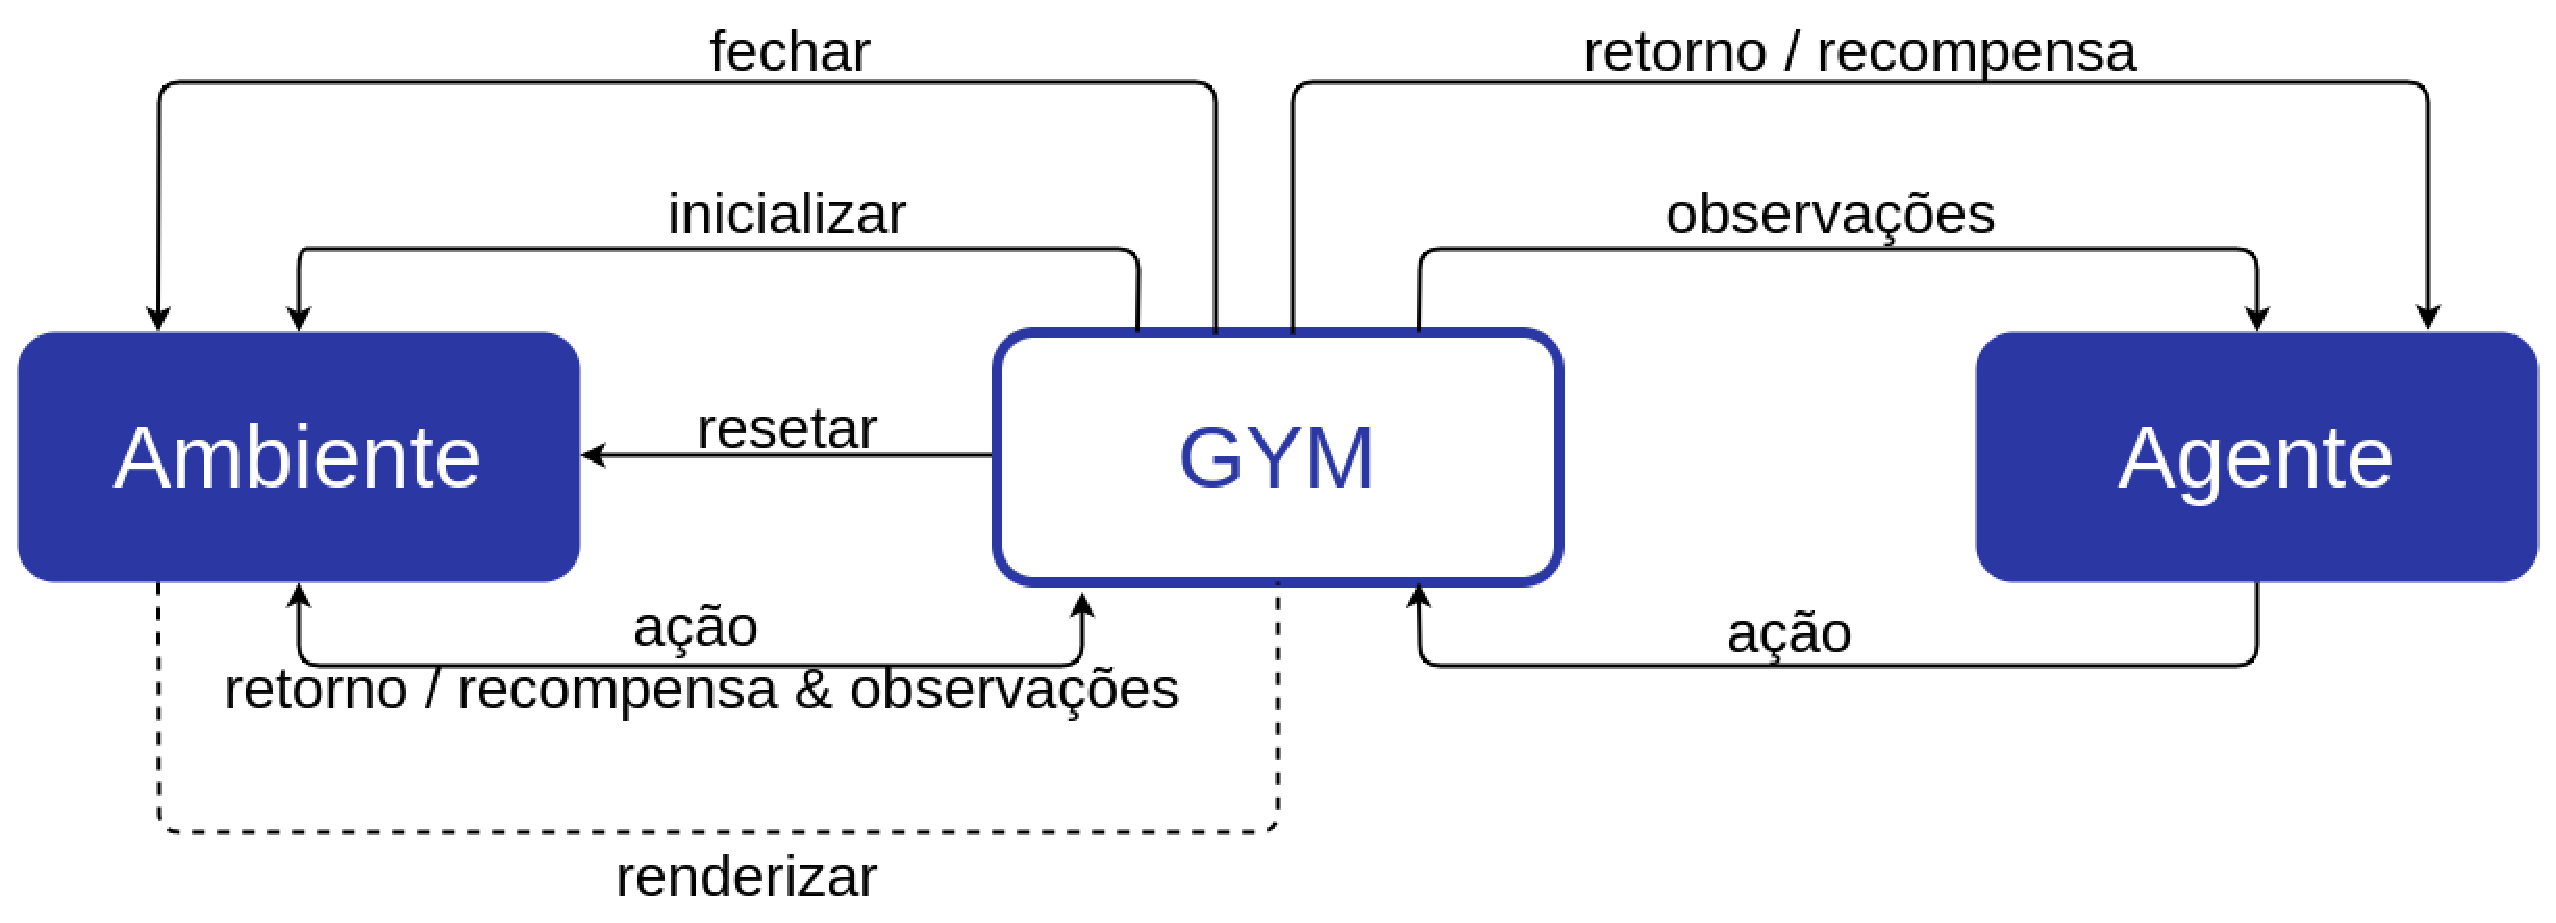
\includegraphics[width=0.9\textwidth]{./fig/gym}
 \caption{Fluxo de funcionamento da ferramenta GYM.}
 \label{fig:gym}
\end{figure}

Os jogos disponíveis no GVGAI\_GYM são jogos bidimensionais do tipo arcade. Jogos de arcade, geralmente, possuem níveis de curta duração, controles simples e uma dificuldade crescente, exigindo bons reflexos e pensamento estratégico dos seus jogadores. A Figura \ref{fig:jogosgvgai}\subref{subfig:super} é referente ao jogo \textit{Superman} e a \ref{fig:jogosgvgai}\subref{subfig:super} ao jogo \textit{Wait For Breakfast}, ambos disponíveis no GVGAI\_GYM.

\begin{figure}[ht]
  \centering
  \subfigure[\textit{Superman}]
  {
    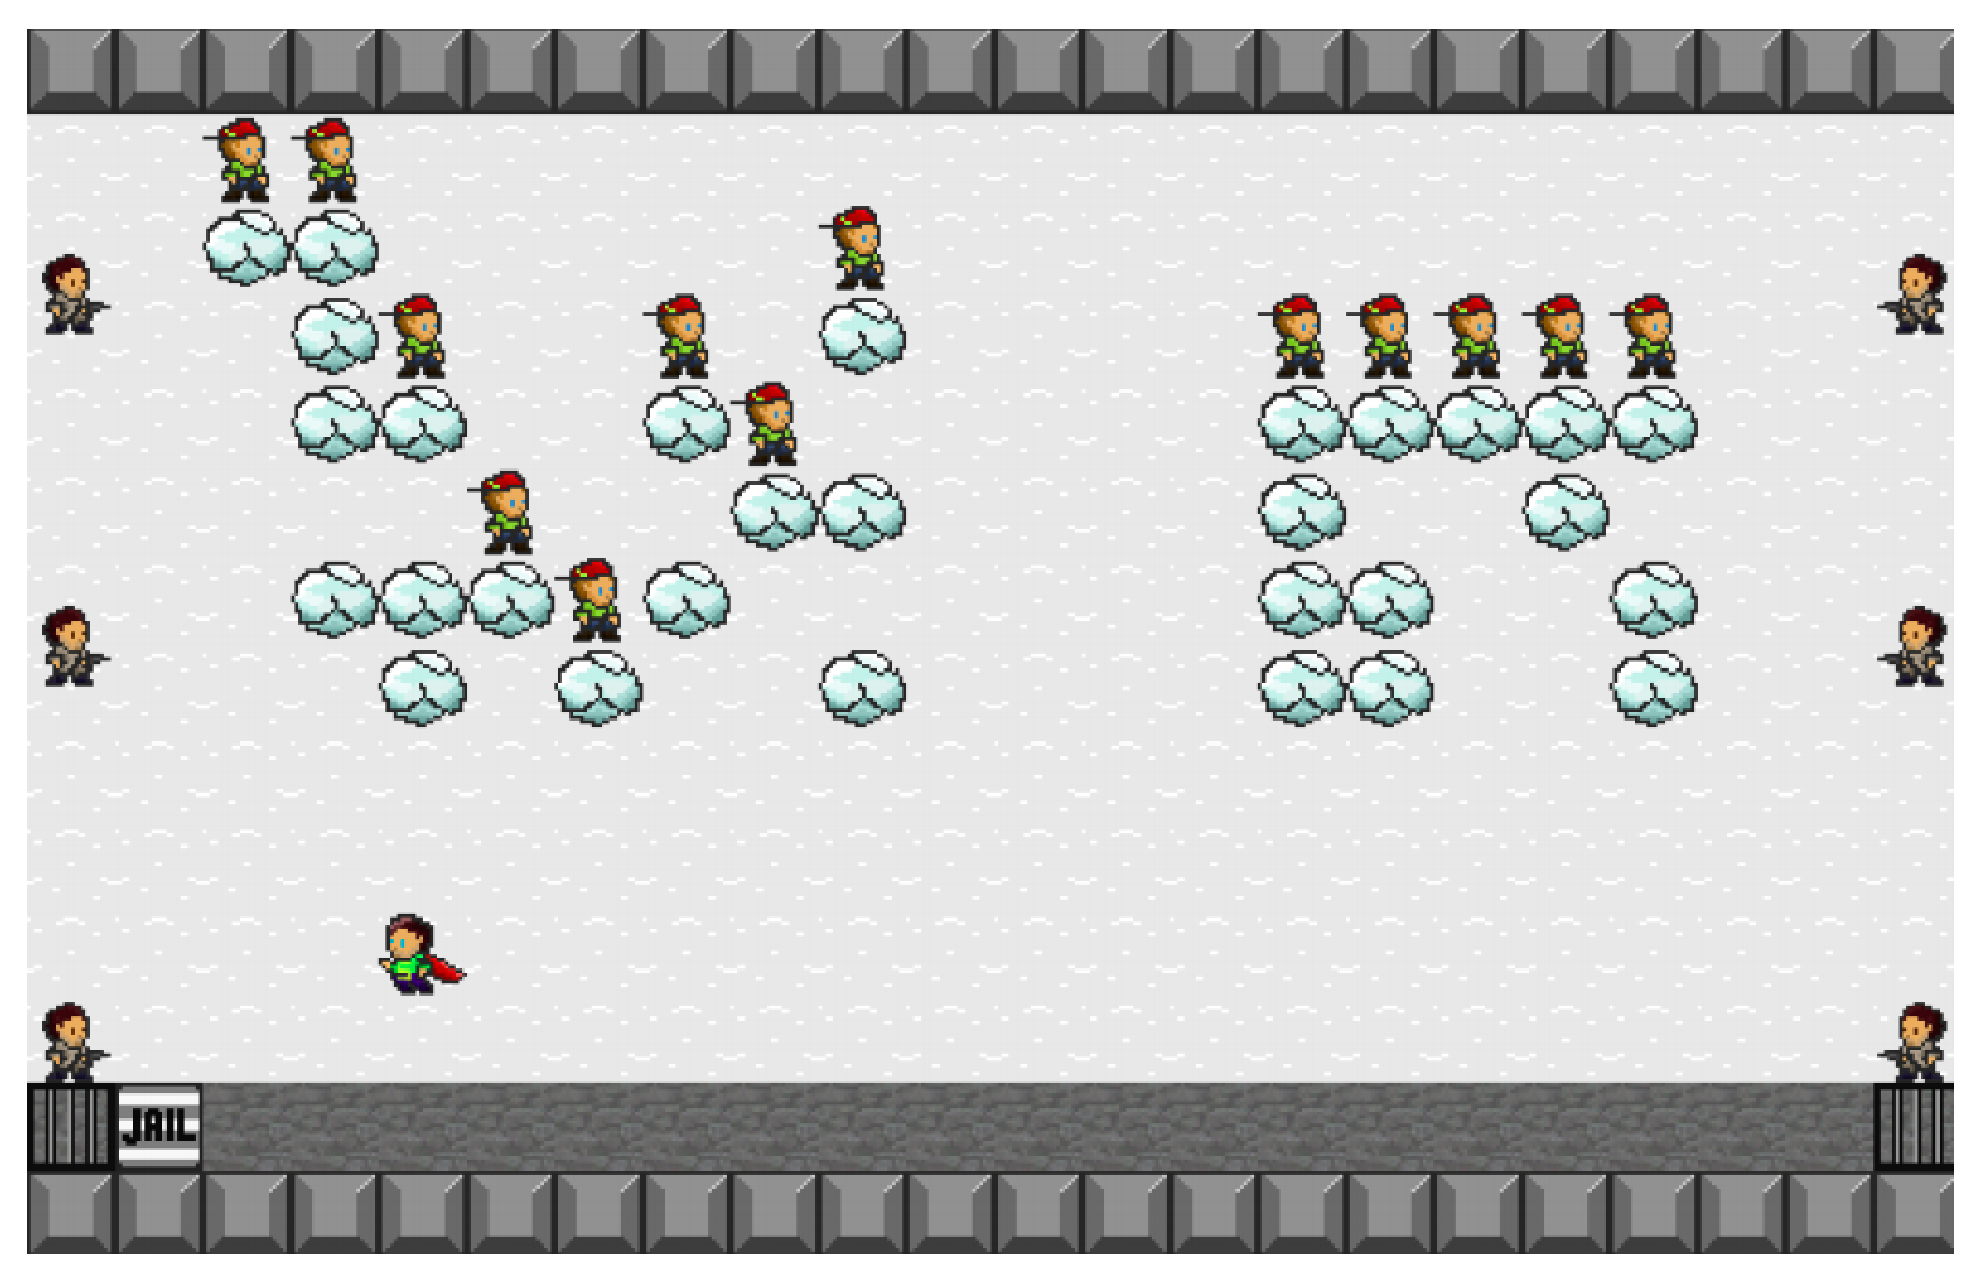
\includegraphics[width=0.42\textwidth]{./fig/superman}
    \label{subfig:super}
  } \qquad
  \subfigure[\textit{Wait For Breakfast}]
  {
    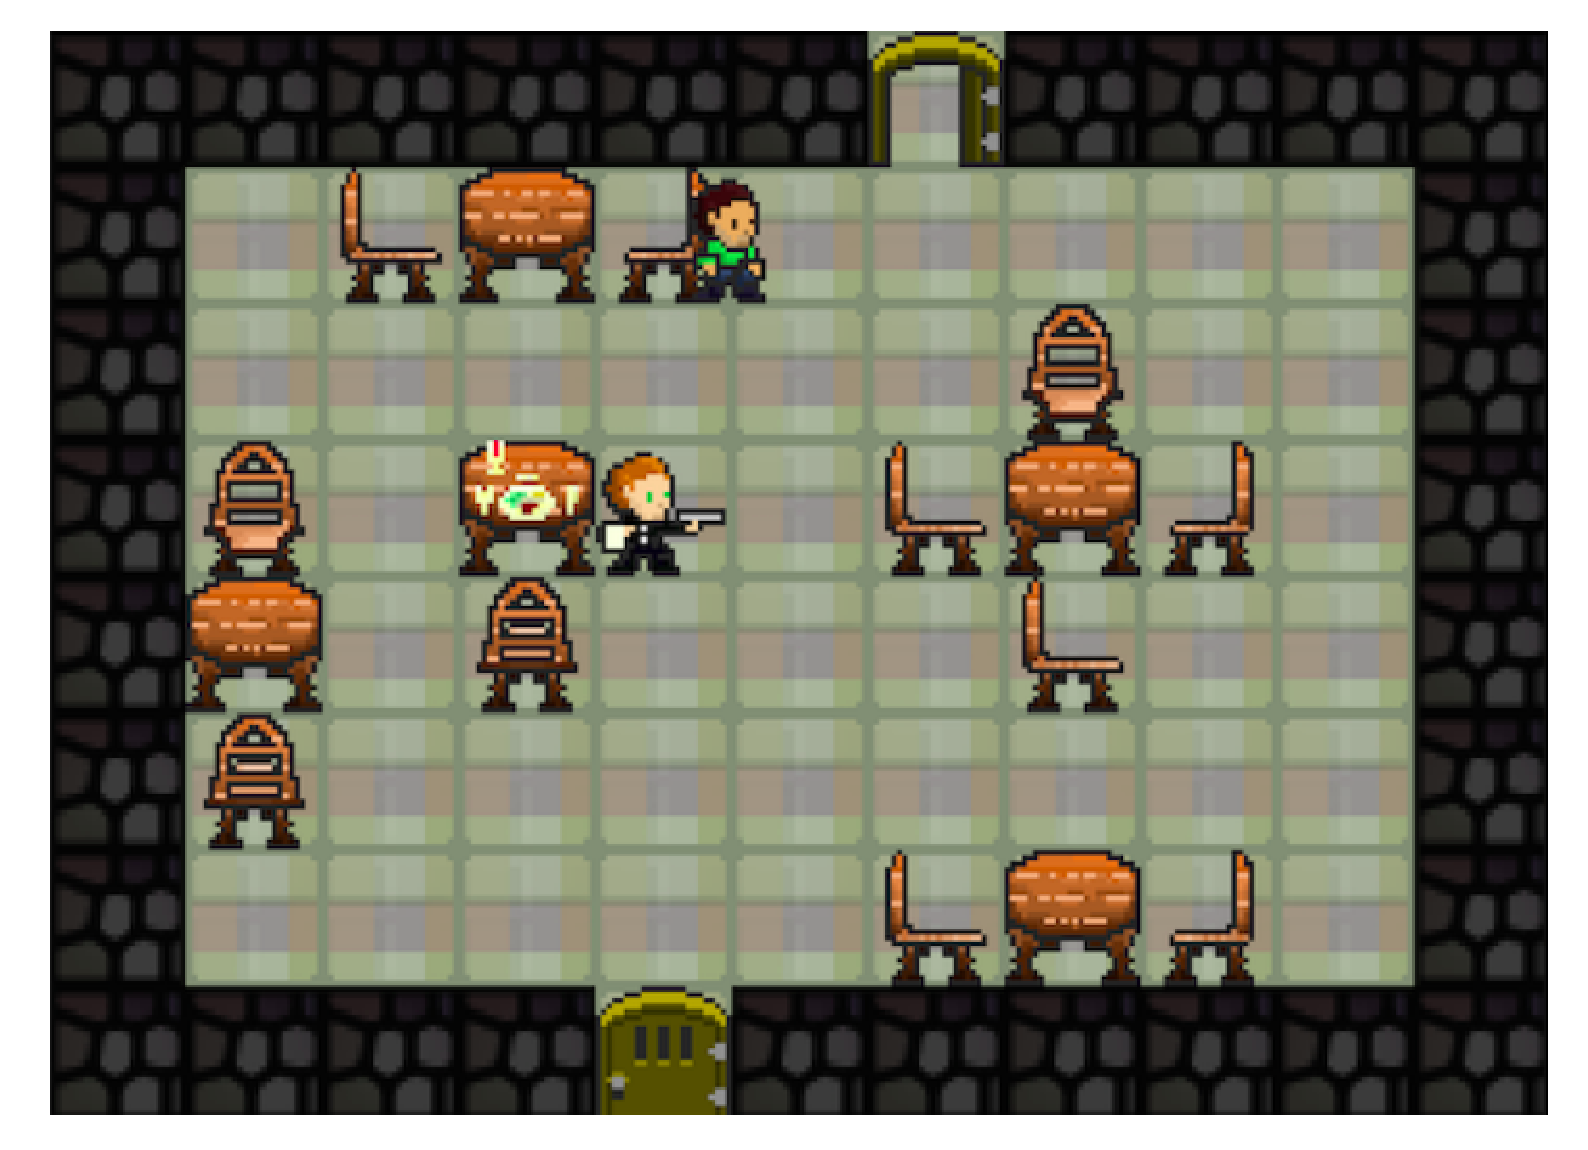
\includegraphics[width=0.38\textwidth]{./fig/waitForBreakfast}
    \label{subfig:wait}
  }
  \caption{Exemplos de jogos disponíveis no GVGAI\_GYM \cite{torrado18}.}
  \label{fig:jogosgvgai}
\end{figure}

% - - - - - - - - - - - - - - - - - - - - - - - - - - - - - - - - - - -

Para os testes da proposta desenvolvida neste trabalho, serão utilizados os jogos \textit{Aliens}, \textit{Boulder Dash} e \textit{Missile Commands}. No primeiro jogo, \textit{Aliens} (Figura \ref{fig:aliens}), as principais tarefas são evitar projéteis inimigos recebidos e disparar no momento certo para atingir o inimigo. Todos os personagens não jogáveis e projéteis se comportam de maneira determinística (projéteis inimigos são disparados estocasticamente, mas leva algum tempo para alcançar o jogador). 

Já no jogo \textit{Boulder Dash} (Figura \ref{fig:boulderdash}), o jogador deve explorar cavernas, coletando diamantes e chegando a uma saída dentro de um prazo, evitando criaturas perigosas e obstáculos. \textit{Boulder Dash} exige que seu jogador possua reações rápidas para evitar quedas de pedras, e planejamento estratégico a longo prazo  para escavar terra e coletar diamantes não ficando preso entre as pedras. 

Por fim, no jogo \textit{Missile Command} (Figura \ref{fig:missilecommand}), cidades estão sendo atacadas por mísseis e o jogador deve destruí-los utilizando os canhões disponíveis. Os mísseis disparados pelo jogador explodem ao atingir a mira, deixando uma bola de fogo que persiste por alguns segundos e destruindo quaisquer mísseis inimigos que entrem nela. Um recompensa positiva é recebida para cada míssil inimigo destruído, e uma recompensa negativa para cada canhão destruído.

\begin{figure}[h]
  \centering
  \subfigure
  {
    
\includegraphics[width=0.39\textwidth]{./fig/gvgai-aliens-lvl0-v0}
    \label{subfig:aliens1}
  } 
  \subfigure
  {
    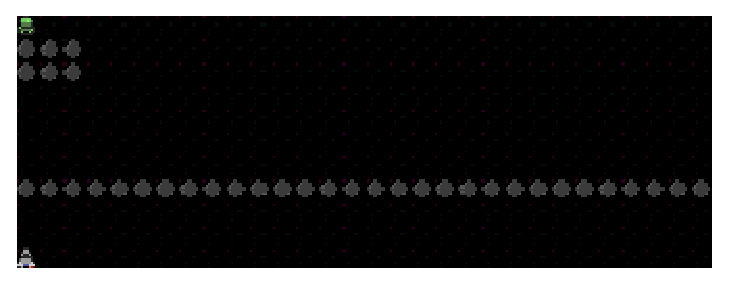
\includegraphics[width=0.39\textwidth]{./fig/gvgai-aliens-lvl4-v0}
    \label{subfig:aliens3}
  }
  \caption{Captura de tela do jogo \textit{Aliens}.}
  \label{fig:aliens}
\end{figure}

\begin{figure}[h]
  \centering
  \subfigure
  {
    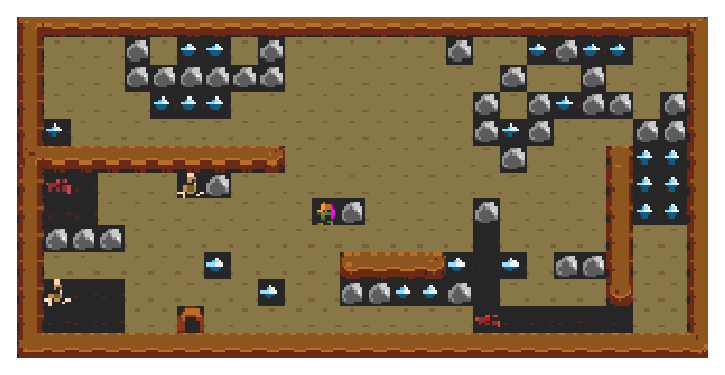
\includegraphics[width=0.39\textwidth]{./fig/gvgai-boulderdash-lvl0-v0}
    \label{subfig:boulderdash1}
  } 
  \subfigure
  {
    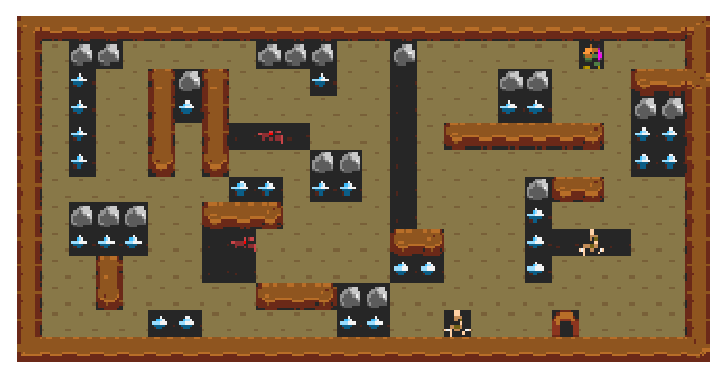
\includegraphics[width=0.39\textwidth]{./fig/gvgai-boulderdash-lvl2-v0}
    \label{subfig:boulderdash3}
  }
  \caption{Captura de tela do jogo \textit{Boulder Dash}.}
  \label{fig:boulderdash}
\end{figure}


\begin{figure}[h]
  \centering
  \subfigure
  {
    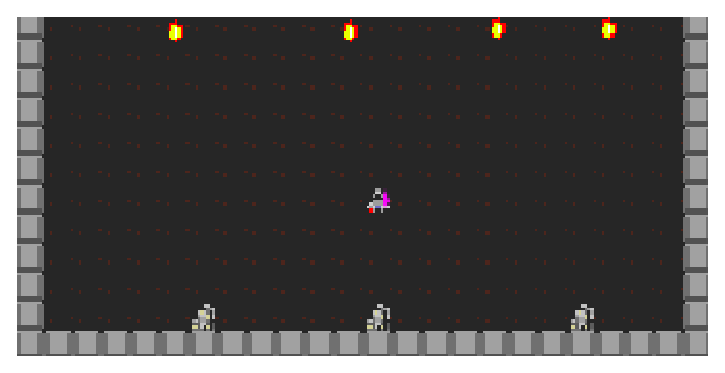
\includegraphics[width=0.39\textwidth]{./fig/gvgai-missilecommand-lvl0-v0}
    \label{subfig:missilecommand1}
  } 
  \subfigure
  {
    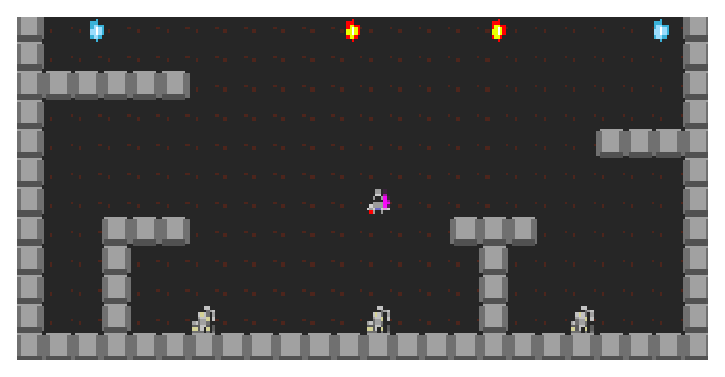
\includegraphics[width=0.39\textwidth]{./fig/gvgai-missilecommand-lvl2-v0}
    \label{subfig:missilecommand3}
  }
  \caption{Captura de tela do jogo \textit{Missile Command}.}
  \label{fig:missilecommand}
\end{figure}

% - - - - - - - - - - - - - - - - - - - - - - - - - - - - - - - - - - -
\section{Algoritmo de Treinamento}

A arquitetura do agente de aprendizado por reforço consiste em duas partes: o algoritmo \textit{Proximal Policy Optimization} e o ambiente de simulação fornecido pelo GVGAI\_GYM. Os ambientes do GVGAI\_GYM se diferenciam em dois aspectos importantes para o agente: o tamanho do espaço de ações disponíveis e o tamanho da imagem do jogo. As imagens são referentes aos estados observáveis do jogo que são passadas para o agente. Para obter dados mais relevantes das observações e tornar o algoritmo mais computacionalmente eficiente, é realizado um pré-processamento nas imagens de entrada. O processo consiste em eliminar as cores presentes na imagem, transformando-a em uma escala de cinza, e redimensionando o tamanho das imagens para o tamanho padrão de $84x84$ \textit{pixels}. A Figura \ref{fig:jogosanalisepp} apresenta a saída do pré-processamento feito sobre uma imagem do jogo. Por fim, é combinado várias imagens em uma única entrada, fazendo com que o modelo escolha ações com base em uma série de quadros em vez de apenas um único quadro. Isso permite ao modelo discernir coisas como a direção do personagem ou sua velocidade.

\begin{figure}[ht]
\centering
  \subfigure[\textit{Aliens}]
  {
    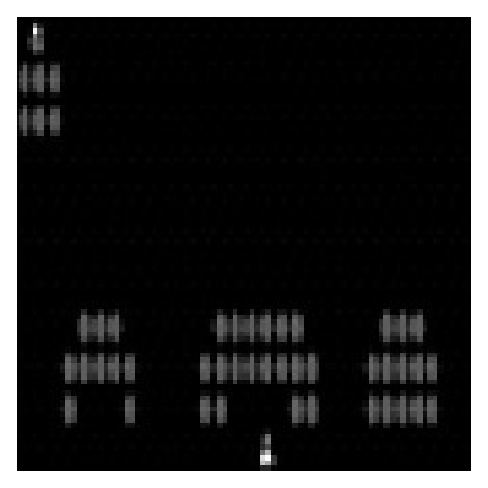
\includegraphics[width=0.3\textwidth]{./fig/alienspp}
    \label{subfig:alienspp}
  } 
  \subfigure[\textit{Boulder Dash}]
  {
    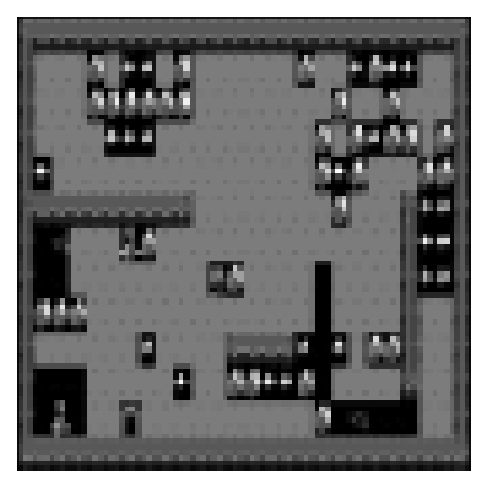
\includegraphics[width=0.3\textwidth]{./fig/boulderdashpp}
    \label{subfig:boudlerdashpp}
  }
  \subfigure[\textit{Missile Commands}]
  {
    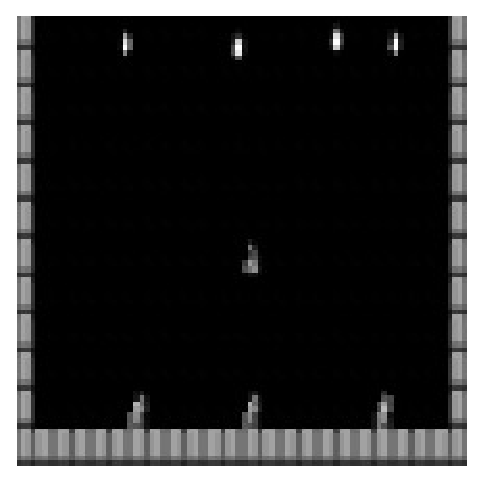
\includegraphics[width=0.3\textwidth]{./fig/missilecommandpp}
    \label{subfig:missilecommandpp}
  }
  \caption{Resultado do pré-processamento das imagens.}
  \label{fig:jogosanalisepp}
\end{figure}

% As imagens pré-processadas são então passadas para o algoritmo \textit{Proximal Policy Optimization} (Seção \ref{section:ppoalg}), que avalia o estado e escolhe uma ação a ser executada. A ação escolhida é passada para o ambiente do GVGAI\_GYM, que então executa a ação no jogo, calcula a recompensa obtida, e retorna o próximo estado. Todo esse processo é repetido até um estado terminal é atingido, indicando que o agente ganhou ou perdeu o jogo, e então o ambiente é reiniciado e o processo começa novamente. para o algoritmo \textit{Proximal Policy Optimization} (Seção \ref{section:ppoalg})

As imagens pré-processadas alimentam duas redes neurais, uma chamada de Ator e outra chamada de Crítico. O modelo Ator é responsável pelo aprendizado de qual ação selecionar a partir de um estado observado do ambiente. Aqui, as imagens do jogo, já pré-processadas, são passadas para uma Rede Neural Convolucional (CNN do inglês \textit{Convolutional Neural Network}) \cite{Krizhevsky12}, que gera como saída uma ação, como andar ou atirar. 

\begin{figure}[ht]
 \centering
  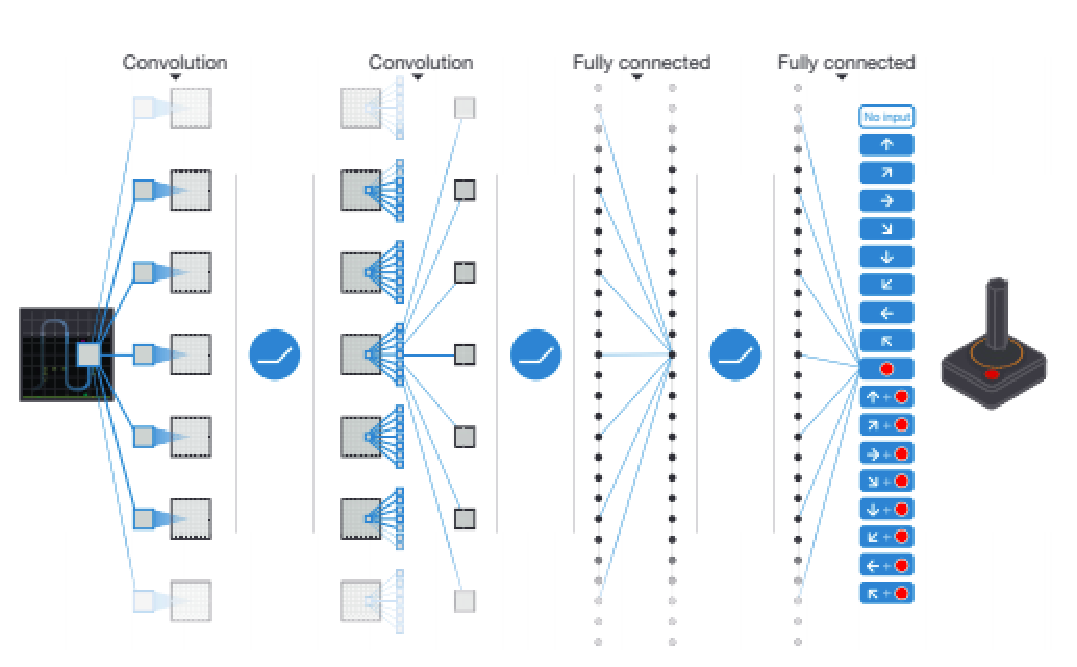
\includegraphics[width=0.8\textwidth]{./fig/cnngame}
  \captionsetup{width=1\textwidth}
 \caption{Ilustração esquemática de uma rede neural convolucional \cite{mnih15}.}
 \label{fig:cnn}
\end{figure}

As ações preditas pelo Ator são passadas para o ambiente do GVGAI\_GYM, que é responsável pela execução da ação no jogo. A ação executada gera uma recompensa que é calculada e retornada juntamente com o próximo estado do jogo. O modelo Crítico deve aprender a avaliar o estado atual, calculando o quão bom o estado é com base em sua recompensa através da função de valor (Função \ref{eqn:value}). Todo esse processo é repetido por uma quantidade finita de passos, em um processo de coleta de trajetórias. Ao final da coleta de trajetórias o valor da função de vantagem (Função \ref{eqn:gae}) é calculado, e os parâmetros do Ator e do Crítico são otimizados com base no Algoritmo \ref{alg:ppoclip}, \textit{Proximal Policy Optimization}. O fluxo de treinamento Ator-Crítico é mostrado na Figura \ref{fig:ac}. As configuração de hiperparâmetros do algoritmo utilizado nos experimentos pode ser conferida no Apêndice \ref{apend:1}, e a implementação do algoritmo pode ser encontrada no Github\footnote{\url{https://github.com/luanagbmartins/general-game-playing}}.

\begin{figure}[ht]
 \centering
  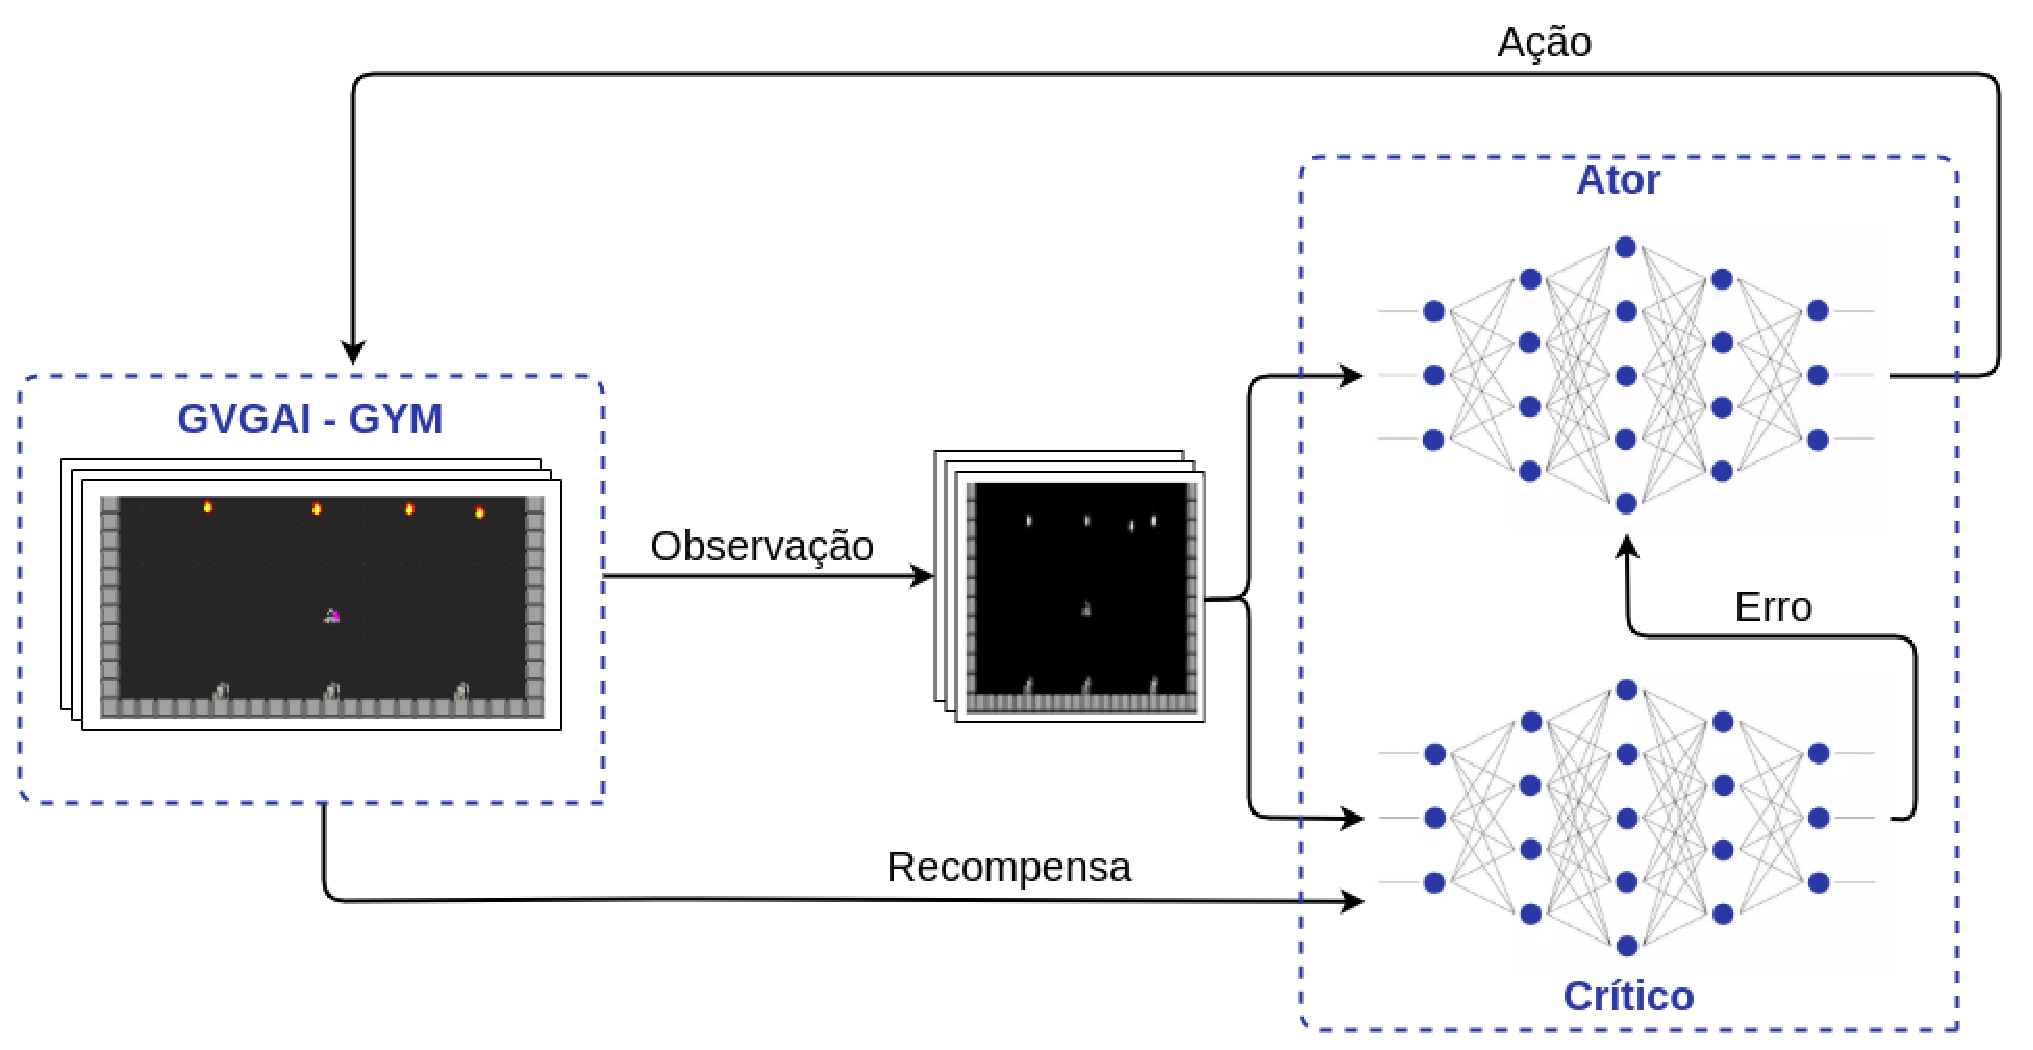
\includegraphics[width=0.92\textwidth]{./fig/ator-critico}
 \caption{Fluxo de treinamento Ator-Crítico.}
 \label{fig:ac}
\end{figure}

% - - - - - - - - - - - - - - - - - - - - - - - - - - - - - - - - - - -
\section{Testes}

Todos os três jogos apresentados na seção anterior são divididos em cinco fases, ou níveis, que serão por sua vez divididos entre conjuntos de treino e teste. Todos os níveis de cada jogo são obtidos da mesma distribuição, portanto a diferença entre o desempenho do conjunto de treinamento e de teste determina o quão super ajustado o agente ficou ao conjunto de treinamento. A medida que o número de níveis de treinamento disponíveis aumenta, espera-se que o desempenho no conjunto de testes melhore, mesmo quando os agentes são treinados para um número fixo de iterações. Para todos os jogos, o treinamento foi limitado a 3 milhões de iterações distribuídas paralelamente entre 8 processos. Cada processo foi responsável por um ambiente do conjunto de treinamento. Os testes de cada jogo foram divididos entre conjuntos de treinamento com uma, duas e três fases. As fases não utilizadas em treinamento irão compor o conjunto de testes utilizados na fase de avaliação do agente.
